\documentclass[10pt]{article}
\usepackage[utf8]{inputenc}
\usepackage[activeacute,spanish]{babel}
\usepackage[left=1.5cm,top=1.5cm,right=1.5cm, bottom=1.5cm,letterpaper, includeheadfoot]{geometry}

\usepackage{amssymb, amsmath, amsthm}
\usepackage{graphicx}
\usepackage{hyperref}
\usepackage{lmodern,url}
\usepackage{paralist} %util para listas compactas
\usepackage{xcolor}
\usepackage{bbm}
\usepackage{mathrsfs}
\usepackage{bbm}

%========PAQUETES AGREGADOS===========
%Pseudocodigo
\usepackage{pseudocode}
\usepackage[portuguese, boxruled]{algorithm2e}
\usepackage{wrapfig}
\usepackage{multicol}
\usepackage{graphicx}
\usepackage{caption}
\usepackage{subcaption}
%\captionsetup[table]{labelformat=empty}
\captionsetup[subfigure]{labelformat=empty}
\usepackage{cancel}
\usepackage{tikz}
\def\checkmark{\tikz\fill[scale=0.4](0,.35) -- (.25,0) -- (1,.7) -- (.25,.15) -- cycle;} 
%====================================

\usepackage{fancyhdr}
\pagestyle{fancy}
\fancypagestyle{plain}{%
\fancyhf{}
\lhead{\footnotesize\itshape\bfseries\rightmark}
\rhead{\footnotesize\itshape\bfseries\leftmark}
}


% macros
\newcommand{\Q}{\mathbb Q}
\newcommand{\R}{\mathbb R}
\newcommand{\N}{\mathbb N}
\newcommand{\Z}{\mathbb Z}
\newcommand{\C}{\mathbb C}
\newcommand{\BigO}{\mathcal{O}}
%Teoremas, Lemas, etc.
\theoremstyle{plain}
\newtheorem{teo}{Teorema}
\newtheorem{lem}{Lema}
\newtheorem{prop}{Proposición}
\newtheorem{cor}{Corolario}
\newtheorem{obs}{Observación}
\newtheorem{ej}{Ejemplo}
\renewcommand{\qedsymbol}{\rule{0.7em}{0.7em}}
\renewenvironment{proof}{{\bfseries \noindent Demostración}}{ \qed \\}


\theoremstyle{definition}
\newtheorem{defi}{Definición}
% fin macros


\newcommand{\catnum}{9} %numero de catedra
\newcommand{\fecha}{13 de Septiembre 2016 }

%%%%%%%%%%%%%%%%%%

%Macros para este documento
\newcommand{\cin}{\operatorname{cint}}



\begin{document}
%Encabezado
\fancyhead[L]{Facultad de Ciencias Físicas y Matemáticas}
\fancyhead[R]{Universidad de Chile}
\vspace*{-1.2 cm}
\begin{minipage}{0.6\textwidth}
\begin{flushleft}
\hspace*{-0.5cm}\textbf{MA3402-1 Estadística. Primavera 2016}\\
\hspace*{-0.5cm}\textbf{Profesor:} Raul Gouet\\
\hspace*{-0.5cm}\textbf{Escriba:} Manuel Cáceres\\
\hspace*{-0.5cm}\textbf{Fecha:} \fecha
\end{flushleft}
\end{minipage}
\begin{minipage}{0.36\textwidth}
\begin{flushright}

\includegraphics[scale=0.3]{imagenes/fcfm_dcc}
\end{flushright}
\end{minipage}
\bigskip
%Fin encabezado

\begin{center}
\LARGE\textbf{Clase \catnum}
\end{center}
\section{Teoría de Neyman-Pearson}
Elementos:
\begin{itemize}
\item Modelo paramétrico $\mathcal{P} = \{\mathbb{P}_{\theta}\colon \theta \in \Theta\}$
\item Partición de $\Theta$ : $\Theta_{0},\Theta_{1}$
\item Hipótesos en competencia: $H_{0}: \theta \in \Theta_{0}$ versus $H_{1}: \theta \in \Theta_{1}$
\item Test de hipótesis: $\Phi: \mathfrak{X} \mapsto \{0,1\}$, donde $\Phi(x) = 1\Rightarrow$ rechazar $H_{0}$, $\Phi(x) = 1\Rightarrow$ no rechazar
\item Región crítica o de rechazo $\mathbb{R}_{\Phi} = \Phi^{-1}(1) = \{x \in \mathbb{X}\colon \Phi(x) = 1\}$
\item Error tipo I (rechazo $H_{0}$ siendo cierto) y tipo II (no rechazo $H_{0}$, siendo falsa)
\item Probabilidad de rechazo como función de $\theta$, $\alpha_{\Phi}(\theta) = \mathbb{P}_{\theta}(x \in \mathbb{R}_{\Phi}) = \mathbb{E}_{\theta}(\Phi)(x))$, con $\alpha_{\Phi}$ discriminamos entre distintos test. La situación ideal sería que $\alpha_{\Phi}(\theta) \approx 0$ si $\theta \in \Theta_{0}$ y $\alpha_{\Phi}(\theta) \approx 1$ si $\theta \in \Theta_{1}$
\end{itemize}
El problema es que al disminuir $\alpha_{\Phi}(\theta), \theta \in \Theta_{0}$ también disminuyo $\alpha_{\Phi}(\theta), \theta \in \Theta_{1}$.\\

Se define la potencia de $\Phi$ como la restricción de $\alpha_{\Phi}$ a $\Theta_{1}$. Un buen test tiene \textbf{potencia alta}.\\

Neyman-Pearson reconocen que el error de tipo I es más grave que el de tipo II (esto incide en la forma que particionamos $\Theta$) y proponen acotar su probabilidad.\\
Con esto se define la clase de test de nivel $\alpha \in [0,1]$
\begin{defi} Se dice que $\Phi$ tiene nivel $\alpha \in [0,1]$ si $\alpha_{\Phi}(\theta) \le \alpha, \forall \theta \in \Theta_{0}$
\end{defi}
\begin{defi} El tamaño de $\Phi$ se define como $\sup_{\theta \in \Theta_{0}} \alpha_{\Phi}(\theta)$
\end{defi}
Designemos $\tau_{\alpha} = \{\Phi\colon \Phi\ test\ y\ \alpha\_{Phi}(\theta) \le \alpha, \forall \theta \in \Theta_{0}\}$, la colección de todos los test de nivel $\alpha \in [0,1]$
\section{Comparación de tests}
Digamos que $\Phi_{1}$ es mejor que $\Phi_{2}$ si 
\begin{align*}
\alpha_{\Phi_{1}}(\theta) \le \alpha_{\Phi_{2}}(\theta)\ \forall \theta \in \Theta_{0}\\
\alpha_{\Phi_{1}}(\theta) \ge \alpha_{\Phi_{2}}(\theta)\ \forall \theta \in \Theta_{1}\\
\end{align*}
\begin{center}
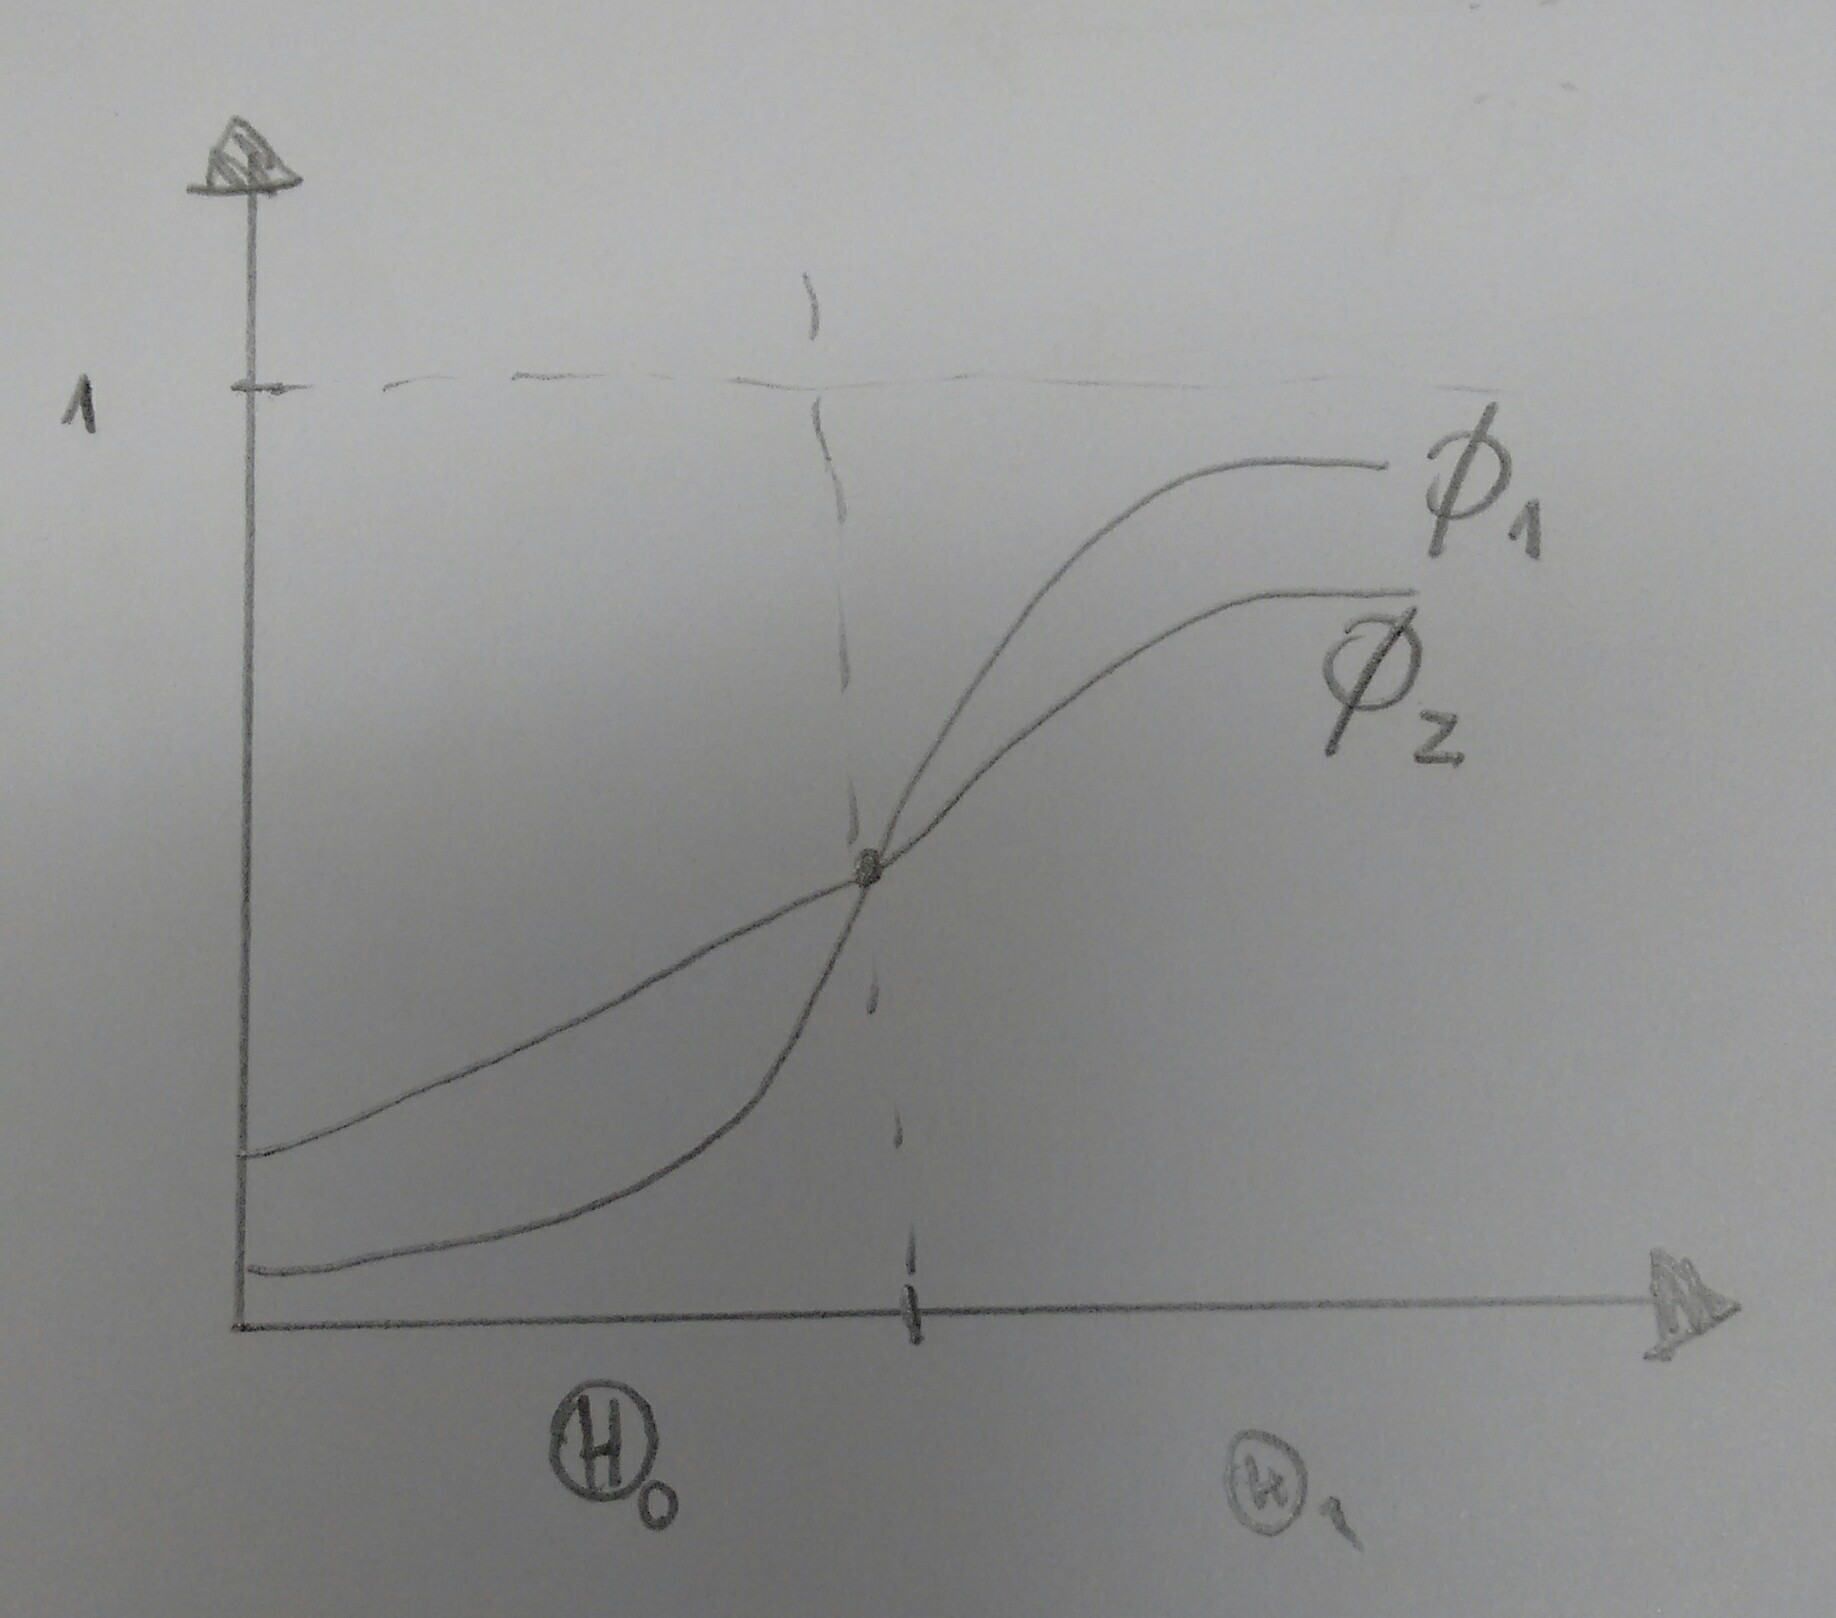
\includegraphics[scale=0.2]{imagenes/test2.jpg}
\end{center}
$\Phi^*$ es el mejor de todos que satisface $\Phi^*$ mejor que $\Phi, \forall \Phi$. No existe!(salvo casos triviales).\\
Para descartar tests observados $\Phi = 0\ o \ = 1$ imponemos la restricción de niveles. Declaramos óptimo al test de nivel $\alpha$ que tenga la mayor potencia.
\begin{defi} Test uniformemente más potente.\\
Se dice que $\Phi^* \in \tau_{\alpha}$ es un test UMP (de nivel $\alpha$) si
\begin{align*}
\alpha_{\Phi^*}(\theta) \ge \alpha_{\Phi}(\theta), \forall \theta \in \Theta_{1}, \forall \Phi \in \tau_{\alpha}
\end{align*}
\end{defi}
\textbf{PROBLEMA: } Dados $H_{0}, H_{1}$ encontrar el/los test UMP de nivel $\alpha$.\\

Vamos a explorar primero un caso de interés académico que es la base ára explorar otras situaciones más complejas.\\
Consideremos $H_{0}: \theta \in \Theta_{0}$ versus $H_{1}: \theta \in \Theta_{1}$.\\

Si $\Theta_{i} = \{\theta_{i}\}$, diremos que $H_{i}$ es una hipótesis simple, de lo contrario diremos que es compuesta.\\

El lema de Neyman-Pearson presenta un test UMP de nivel $\alpha$ para $H_{0},H_{1}$ hipótesis simple.\\

\textbf{Contexto para el LNP:} Consideremos un modelo paramétrico con $\Theta = \{\theta_{0}, \theta_{1}\}, \theta{0}\not =\theta_{1}$ y dominado, es decir, $X$ tiene densidad $f_{\theta}(x)$(discreta o continua). Adoptemos la notación $f_{i}(x) := f_{\theta_{i}}(x)$.\\
A continuación presentamos el célebre test de Neyman-Pearson(NP) de nivel $\alpha$.\\

Dado $\alpha \in [0,1]$ se define el conjunto $\mathbb{R}^* = \{x\in\mathfrak{X}\colon f_{1}(x) \ge k_{\alpha}f_{0}(x)\}$, donde $k_{\alpha}$ es una constante que se calcula imponiendo una restricción para el test $\Phi^*$(TNP), cuya región crítica es $\mathbb{R}^*$ .\\

Es decir, $\Phi^*$ tiene como región crítica a $\mathbb{R}^*$ ssi $\Phi^*(x)=\mathbbm{1}_{\{x\in \mathbbm{R}^*\}} = \mathbbm{\mathbb{R}^*}(\alpha)$\\

El umbral $k_{\alpha}$ se calcula de manera que $\mathbb{P}_{\theta}(x\in\mathbb{R}^*) = \mathbb{E}_{\theta_{0}}(\Phi^*(x))=\alpha$.\\

Claramente, si $\exists k_{\alpha}$, entonces $\Phi^* \in \tau_{\alpha}$. Pero $k_{\alpha}$ podría no existir si es que por ejemplo la distribución de datos es discontinua($X$ discreto).
\begin{lem}
Sea $\Phi^*$ definida más arriba. Entonces
\begin{align*}
\alpha_{\Phi^*}(\theta_{1}) \ge \alpha_{\Phi}(\theta_{1}), \forall \Phi \in \tau_{\alpha}
\end{align*}
\end{lem}
\begin{proof}
Veamos que
\begin{align*}
\alpha_{\Phi^*}(\theta_{1}) - \alpha_{\Phi}(\theta_{1}) \ge 0, \forall \Phi \in \tau_{\alpha}
\end{align*}
Reescribimos
\begin{align*}
\alpha_{\Phi^*}(\theta_{1}) - \alpha_{\Phi}(\theta_{1}) = \mathbb{P}_{\theta_{1}}(x\in\mathbb{R}^*) -\mathbb{P}_{\theta_{1}}(x\in\mathbb{R})
\end{align*}
Notamos que 
\begin{align*}
\mathbb{P}_{\theta}(x \in \mathbb{R}^*) &= \mathbb{P}_{\theta}(x\in \mathbb{R}^* \cap \mathbb{R}) + \mathbb{P}_{\theta}(x\in \mathbb{R}^* \cap \bar{\mathbb{R}})\\
\mathbb{P}_{\theta}(x \in \mathbb{R}) &= \mathbb{P}_{\theta}(x\in \mathbb{R} \cap \mathbb{R}^*) + \mathbb{P}_{\theta}(x\in \mathbb{R} \cap \bar{\mathbb{R}^*})
\end{align*}
Luego
\begin{align*}
\alpha_{\Phi^*}(\theta_{1}) - \alpha_{\Phi}(\theta_{1}) &= \mathbb{P}_{\theta_{1}}(x\in \mathbb{R}^* \cap \bar{\mathbb{R}}) - \mathbb{P}_{\theta_{1}}(x\in \mathbb{R} \cap \bar{\mathbb{R}^*})\\
&=\int_{\mathbb{R}^* \cap \bar{\mathbb{R}}} {f_{1}(x)dx} - \int_{\mathbb{R}^* \cap \bar{\mathbb{R}^*}} {f_{1}(x)dx}\\
&\ge \int_{\mathbb{R}^* \cap \bar{\mathbb{R}}} {k_{\alpha}f_{0}(x)dx} - \int_{\mathbb{R}^* \cap \bar{\mathbb{R}^*}} {k_{\alpha}f_{0}(x)dx}\\
&= k_{\alpha}\left(\int_{\mathbb{R}^* \cap \bar{\mathbb{R}}} {f_{0}(x)dx} - \int_{\mathbb{R}^* \cap \bar{\mathbb{R}^*}} {f_{0}(x)dx}\right)\\
&=k_{\alpha}\left(\underbrace{\mathbb{P}_{\theta_{0}}(x\in\mathbb{R}^*)}_{=\alpha}-\underbrace{\mathbb{P}_{\theta_{0}}(x\in\mathbb{R})}_{\le \alpha}\right)\\
&\ge 0
\end{align*}
\end{proof}
\begin{ej}
Sea $X=(X_{1},X_{2},\ldots,X_{n})$ iid $N(\mu,\sigma^)$, $\sigma$ conocido.\\
Suponemos que $\mu \in \{\mu_{0},\mu_{1}\}= \Theta$ \\
Consideremos $H_{0}: \mu = \mu_{0}$ y $H_{1}: \mu = \mu_{1}$ y supongamos $\mu_{0}\not = \mu_{1}$.\\

Desarrollemos el TNP, tenemos
\begin{align*}
f_{\mu_{i}}(x) = f_{i}(x) &= \left(\frac{1}{\sqrt{2\pi}\sigma}\right)^n e^{-\frac{1}{2\sigma^2}\sum_{j=1}^n{(x_{j}-\mu_{i})^2}}\ge 0\\
\mathbb{R}^* &= \left\lbrace x \in\mathfrak{X}\colon \lambda(x) = e^{-\frac{1}{2\sigma^2}\left(\sum{(x_{j}-\mu_{1})^2}-\sum{(x_{j}-\mu_{0})^2}\right)} \ge k_{\alpha}\right\rbrace
\end{align*}
Vamos simpleficando la descripción de los $\mathbb{R}^*$
\begin{align*}
\lambda(x) \ge k_{\alpha} \Leftrightarrow &\sum{(x_{j}-\mu_{1})^2}-\sum{(x_{j}-\mu_{0})^2} \le k_{\alpha}'\\
\Leftrightarrow & 2\sum{x_{j}(\mu_{0}-\mu_{1})} + n(\mu_{1}^2-\mu_{0}^2) \le k_{\alpha}'\\
\Leftrightarrow & \frac{1}{n} \sum {nx_{j}(\mu_{0}-\mu_{1})} \le k_{\alpha}''\\
\Leftrightarrow & \bar{X} \ge k_{\alpha}'''\\
\Leftrightarrow & x \in \mathbb{R}^*
\end{align*}
Entonces imponemos
\begin{align*}
\mathbb{P}_{\mu_{0}}(x \in \mathbb{R}^*) = \mathbb{P}_{\mu_{0}}(\bar{X} \ge k_{\alpha}''') = \alpha
\end{align*}
Sabemos que si estamos bajo $H_{0}$, $\bar{X}\sim N(\mu_{0},\sigma^2/n)$ y por lo tanto, $\frac{\bar{X}-\mu_{0}}{\sigma/\sqrt{n}} \sim N(0,1)$.\\

Es decir,
\begin{align*}
&\mathbb{P}_{\mu_{0}}(x \in \mathbb{R}^*) = \mathbb{P}_{\mu_{0}}(\frac{\bar{X}-\mu_{0}}{\sigma/\sqrt{n}} \ge \frac{k_{\alpha}'''-\mu_{0}}{\sigma/\sqrt{n}}) = \alpha \\
\Leftrightarrow & 1-\Phi\left(\frac{k_{\alpha}'''-\mu_{0}}{\sigma/\sqrt{n}}\right) = \alpha\\
\Leftrightarrow & \frac{k_{\alpha}'''-\mu_{0}}{\sigma/\sqrt{n}} = \Phi^{-1}(1-\alpha)\\
\Rightarrow & k_{\alpha}''' = \sigma/\sqrt{n} \Phi^{-1}(1-\alpha) + \mu_{0}\\
\Rightarrow & \mathbb{R}^* = \{x\in\mathfrak{X}\colon \bar{X}\ge\sigma/\sqrt{n} \Phi^{-1}(1-\alpha) + \mu_{0}\}
\end{align*}
\end{ej}
\end{document}
